\documentclass{standalone}
\usepackage{tikz}
\usetikzlibrary{patterns, positioning}


\begin{document}
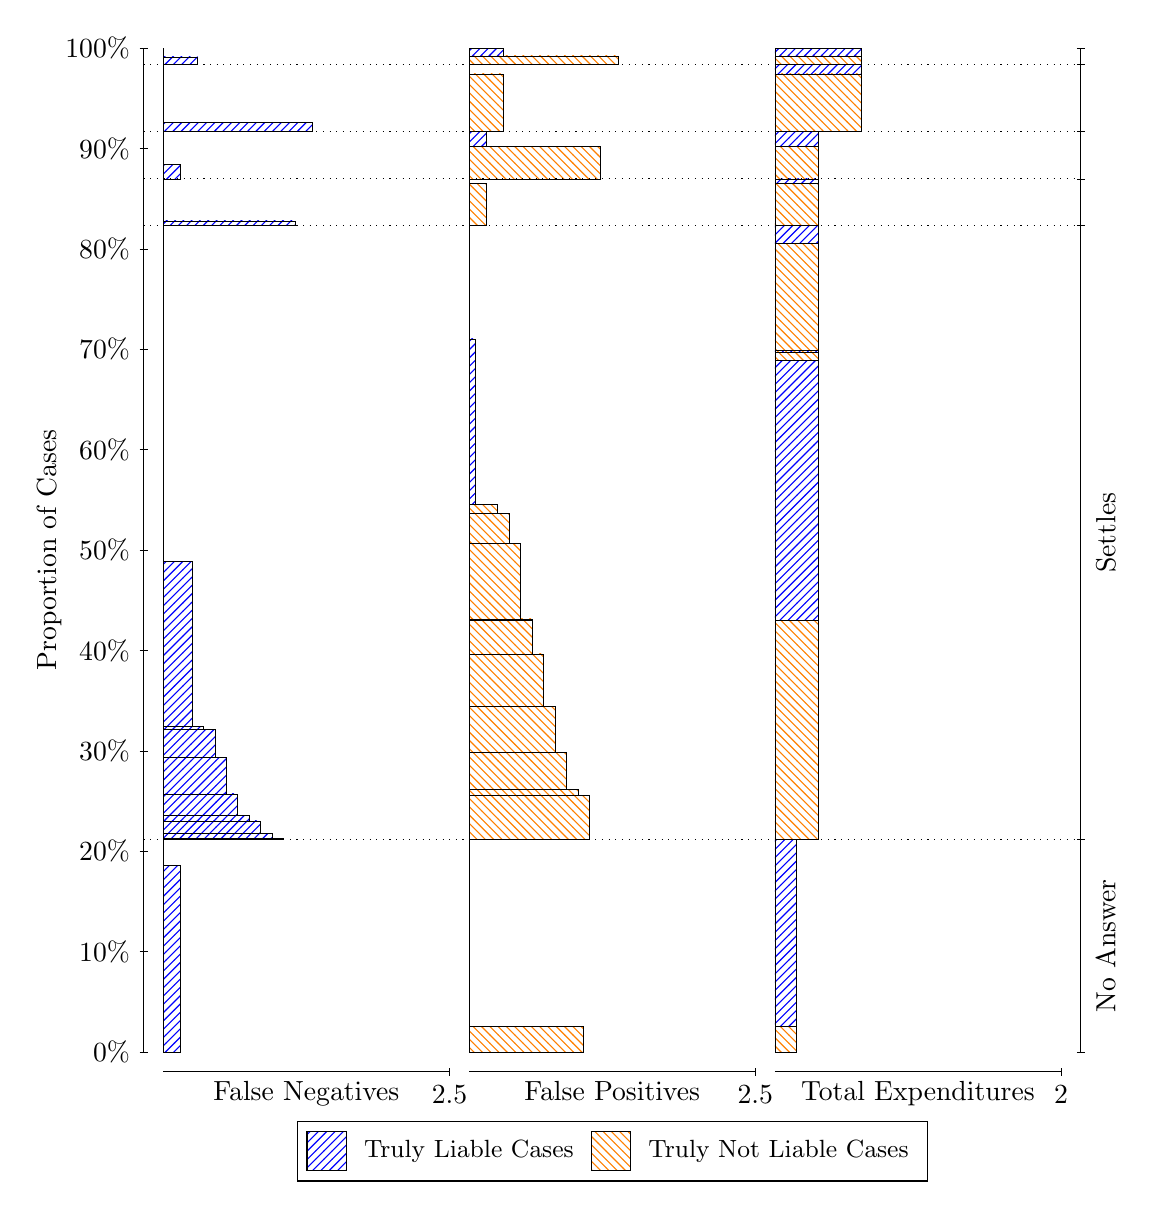
\begin{tikzpicture}
\draw[black, very thin] (1.5,1.75) -- (1.5,14.5);
\node[rotate=90, text=black, anchor=center] at (0.3, 8.125) {Proportion of Cases};
\draw[black, very thin] (1.45,1.75) -- (1.55,1.75);
\node[text=black, anchor=east] at (1.45, 1.75) {0\%};
\draw[black, very thin] (1.45,3.025) -- (1.55,3.025);
\node[text=black, anchor=east] at (1.45, 3.025) {10\%};
\draw[black, very thin] (1.45,4.3) -- (1.55,4.3);
\node[text=black, anchor=east] at (1.45, 4.3) {20\%};
\draw[black, very thin] (1.45,5.575) -- (1.55,5.575);
\node[text=black, anchor=east] at (1.45, 5.575) {30\%};
\draw[black, very thin] (1.45,6.85) -- (1.55,6.85);
\node[text=black, anchor=east] at (1.45, 6.85) {40\%};
\draw[black, very thin] (1.45,8.125) -- (1.55,8.125);
\node[text=black, anchor=east] at (1.45, 8.125) {50\%};
\draw[black, very thin] (1.45,9.4) -- (1.55,9.4);
\node[text=black, anchor=east] at (1.45, 9.4) {60\%};
\draw[black, very thin] (1.45,10.675) -- (1.55,10.675);
\node[text=black, anchor=east] at (1.45, 10.675) {70\%};
\draw[black, very thin] (1.45,11.95) -- (1.55,11.95);
\node[text=black, anchor=east] at (1.45, 11.95) {80\%};
\draw[black, very thin] (1.45,13.225) -- (1.55,13.225);
\node[text=black, anchor=east] at (1.45, 13.225) {90\%};
\draw[black, very thin] (1.45,14.5) -- (1.55,14.5);
\node[text=black, anchor=east] at (1.45, 14.5) {100\%};

\draw[black, very thin] (13.4,1.75) -- (13.4,14.5);
\draw[black, very thin] (13.35,1.75) -- (13.45,1.75);
\node[anchor=west] at (13.35, 1.75) {};
\draw[black, very thin] (13.35,4.4455) -- (13.45,4.4455);
\node[anchor=west] at (13.35, 4.4455) {};
\draw[black, very thin] (13.35,12.244) -- (13.45,12.244);
\node[anchor=west] at (13.35, 12.244) {};
\draw[black, very thin] (13.35,12.838) -- (13.45,12.838);
\node[anchor=west] at (13.35, 12.838) {};
\draw[black, very thin] (13.35,13.437) -- (13.45,13.437);
\node[anchor=west] at (13.35, 13.437) {};
\draw[black, very thin] (13.35,14.288) -- (13.45,14.288);
\node[anchor=west] at (13.35, 14.288) {};
\draw[black, very thin] (13.35,14.5) -- (13.45,14.5);
\node[anchor=west] at (13.35, 14.5) {};

\draw[black, very thin, pattern color=blue, pattern=north east lines] (1.75,1.75) rectangle (1.968,4.1213);
\draw[black, very thin, pattern color=orange, pattern=north west lines] (1.75,4.1213) rectangle (1.75,4.4455);
\draw[black, very thin, pattern color=blue, pattern=north east lines] (1.75,4.4455) rectangle (3.276,4.462);
\draw[black, very thin, pattern color=blue, pattern=north east lines] (1.75,4.462) rectangle (3.1307,4.5242);
\draw[black, very thin, pattern color=blue, pattern=north east lines] (1.75,4.5242) rectangle (2.9853,4.6847);
\draw[black, very thin, pattern color=blue, pattern=north east lines] (1.75,4.6847) rectangle (2.84,4.7567);
\draw[black, very thin, pattern color=blue, pattern=north east lines] (1.75,4.7567) rectangle (2.6947,5.0277);
\draw[black, very thin, pattern color=blue, pattern=north east lines] (1.75,5.0277) rectangle (2.5493,5.4883);
\draw[black, very thin, pattern color=blue, pattern=north east lines] (1.75,5.4883) rectangle (2.404,5.8436);
\draw[black, very thin, pattern color=blue, pattern=north east lines] (1.75,5.8436) rectangle (2.2587,5.8835);
\draw[black, very thin, pattern color=blue, pattern=north east lines] (1.75,5.8835) rectangle (2.1133,7.9848);
\draw[black, very thin, pattern color=orange, pattern=north west lines] (1.75,7.9848) rectangle (1.75,12.244);
\draw[black, very thin, pattern color=blue, pattern=north east lines] (1.75,12.244) rectangle (3.4213,12.304);
\draw[black, very thin, pattern color=orange, pattern=north west lines] (1.75,12.304) rectangle (1.75,12.838);
\draw[black, very thin, pattern color=blue, pattern=north east lines] (1.75,12.838) rectangle (1.968,13.027);
\draw[black, very thin, pattern color=orange, pattern=north west lines] (1.75,13.027) rectangle (1.75,13.437);
\draw[black, very thin, pattern color=blue, pattern=north east lines] (1.75,13.437) rectangle (3.6393,13.553);
\draw[black, very thin, pattern color=orange, pattern=north west lines] (1.75,13.553) rectangle (1.75,14.288);
\draw[black, very thin, pattern color=blue, pattern=north east lines] (1.75,14.288) rectangle (2.186,14.387);
\draw[black, very thin, pattern color=orange, pattern=north west lines] (1.75,14.387) rectangle (1.75,14.5);
\draw[black, very thin, pattern color=orange, pattern=north west lines] (5.6333,1.75) rectangle (7.0867,2.0742);
\draw[black, very thin, pattern color=blue, pattern=north east lines] (5.6333,2.0742) rectangle (5.6333,4.4455);
\draw[black, very thin, pattern color=orange, pattern=north west lines] (5.6333,4.4455) rectangle (7.1593,5.0054);
\draw[black, very thin, pattern color=orange, pattern=north west lines] (5.6333,5.0054) rectangle (7.014,5.0848);
\draw[black, very thin, pattern color=orange, pattern=north west lines] (5.6333,5.0848) rectangle (6.8687,5.5509);
\draw[black, very thin, pattern color=orange, pattern=north west lines] (5.6333,5.5509) rectangle (6.7233,6.1406);
\draw[black, very thin, pattern color=orange, pattern=north west lines] (5.6333,6.1406) rectangle (6.578,6.8053);
\draw[black, very thin, pattern color=orange, pattern=north west lines] (5.6333,6.8053) rectangle (6.4327,7.2329);
\draw[black, very thin, pattern color=orange, pattern=north west lines] (5.6333,7.2329) rectangle (6.4327,7.2493);
\draw[black, very thin, pattern color=orange, pattern=north west lines] (5.6333,7.2493) rectangle (6.2873,8.2115);
\draw[black, very thin, pattern color=orange, pattern=north west lines] (5.6333,8.2115) rectangle (6.142,8.5925);
\draw[black, very thin, pattern color=orange, pattern=north west lines] (5.6333,8.5925) rectangle (5.9967,8.7047);
\draw[black, very thin, pattern color=blue, pattern=north east lines] (5.6333,8.7047) rectangle (5.706,10.806);
\draw[black, very thin, pattern color=blue, pattern=north east lines] (5.6333,10.806) rectangle (5.6333,12.244);
\draw[black, very thin, pattern color=orange, pattern=north west lines] (5.6333,12.244) rectangle (5.8513,12.777);
\draw[black, very thin, pattern color=blue, pattern=north east lines] (5.6333,12.777) rectangle (5.6333,12.838);
\draw[black, very thin, pattern color=orange, pattern=north west lines] (5.6333,12.838) rectangle (7.3047,13.248);
\draw[black, very thin, pattern color=blue, pattern=north east lines] (5.6333,13.248) rectangle (5.8513,13.437);
\draw[black, very thin, pattern color=orange, pattern=north west lines] (5.6333,13.437) rectangle (6.0693,14.172);
\draw[black, very thin, pattern color=blue, pattern=north east lines] (5.6333,14.172) rectangle (5.6333,14.288);
\draw[black, very thin, pattern color=orange, pattern=north west lines] (5.6333,14.288) rectangle (7.5227,14.401);
\draw[black, very thin, pattern color=blue, pattern=north east lines] (5.6333,14.401) rectangle (6.0693,14.5);
\draw[black, very thin, pattern color=orange, pattern=north west lines] (9.5167,1.75) rectangle (9.7892,2.0742);
\draw[black, very thin, pattern color=blue, pattern=north east lines] (9.5167,2.0742) rectangle (9.7892,4.4455);
\draw[black, very thin, pattern color=orange, pattern=north west lines] (9.5167,4.4455) rectangle (10.062,7.2329);
\draw[black, very thin, pattern color=blue, pattern=north east lines] (9.5167,7.2329) rectangle (10.062,10.529);
\draw[black, very thin, pattern color=orange, pattern=north west lines] (9.5167,10.529) rectangle (10.062,10.642);
\draw[black, very thin, pattern color=blue, pattern=north east lines] (9.5167,10.642) rectangle (10.062,10.658);
\draw[black, very thin, pattern color=orange, pattern=north west lines] (9.5167,10.658) rectangle (10.062,12.018);
\draw[black, very thin, pattern color=blue, pattern=north east lines] (9.5167,12.018) rectangle (10.062,12.244);
\draw[black, very thin, pattern color=orange, pattern=north west lines] (9.5167,12.244) rectangle (10.062,12.777);
\draw[black, very thin, pattern color=blue, pattern=north east lines] (9.5167,12.777) rectangle (10.062,12.838);
\draw[black, very thin, pattern color=orange, pattern=north west lines] (9.5167,12.838) rectangle (10.062,13.248);
\draw[black, very thin, pattern color=blue, pattern=north east lines] (9.5167,13.248) rectangle (10.062,13.437);
\draw[black, very thin, pattern color=orange, pattern=north west lines] (9.5167,13.437) rectangle (10.607,14.172);
\draw[black, very thin, pattern color=blue, pattern=north east lines] (9.5167,14.172) rectangle (10.607,14.288);
\draw[black, very thin, pattern color=orange, pattern=north west lines] (9.5167,14.288) rectangle (10.607,14.401);
\draw[black, very thin, pattern color=blue, pattern=north east lines] (9.5167,14.401) rectangle (10.607,14.5);
\draw[black, dotted] (1.5,4.4455) -- (13.4,4.4455);
\draw[black, dotted] (1.5,12.244) -- (13.4,12.244);
\draw[black, dotted] (1.5,12.838) -- (13.4,12.838);
\draw[black, dotted] (1.5,13.437) -- (13.4,13.437);
\draw[black, dotted] (1.5,14.288) -- (13.4,14.288);
\draw[black, very thin] (1.75,1.5) -- (5.3833,1.5);
\node[text=black, anchor=north] at (3.5667, 1.5) {False Negatives};
\draw[black, very thin] (5.3833,1.45) -- (5.3833,1.55);
\node[text=black, anchor=north] at (5.3833, 1.45) {2.5};

\draw[black, very thin] (5.6333,1.5) -- (9.2667,1.5);
\node[text=black, anchor=north] at (7.45, 1.5) {False Positives};
\draw[black, very thin] (9.2667,1.45) -- (9.2667,1.55);
\node[text=black, anchor=north] at (9.2667, 1.45) {2.5};

\draw[black, very thin] (9.5167,1.5) -- (13.15,1.5);
\node[text=black, anchor=north] at (11.333, 1.5) {Total Expenditures};
\draw[black, very thin] (13.15,1.45) -- (13.15,1.55);
\node[text=black, anchor=north] at (13.15, 1.45) {2};

\node[text=black, centered, rotate=90] at (13.72, 3.0977) {No Answer};
\node[text=black, centered, rotate=90] at (13.72, 8.3447) {Settles};





\draw (7.449999999999999,1.5) node[draw=none] (baseCoordinate) {};
\begin{scope}[align=center]
        \matrix[scale=0.5, draw=black, below=0.5cm of baseCoordinate, nodes={draw}, column sep=0.1cm]{
            \node[rectangle, draw, minimum width=0.5cm, minimum height=0.5cm, pattern color=blue, pattern=north east lines] {}; &
            \node[draw=none, font=\small, text=black] (B) {Truly Liable Cases}; &
            \node[rectangle, draw, minimum width=0.5cm, minimum height=0.5cm, pattern color=orange, pattern=north west lines] {}; &
            \node[draw=none, font=\small, text=black] (B) {Truly Not Liable Cases}; \\
            };
\end{scope}

\end{tikzpicture}
\end{document}